%!TEX root = ../../main.tex

\chapter{Theoretische Grundlagen}
In diesem Kapitel sollen die theoretischen Grundlagen erläutert werden. Zunächst wird untersucht, wie das Lernen im Allgemeinen funktioniert und wie diese Erkenntnisse auf das Lernen von Eröffnungen angewendet werden können. Danach wird gezeigt, wie die Lerntechnik Spaced Repetition beim Lernen helfen kann.
Anschließend wird auf die Erkenntnisse im Bereich der Schachpsychologie eingegangen. Dabei wird betrachtet, wie Schachspieler nach heutigem Wissensstand lernen und spielen. Schließlich werden Schnittstellen in Computerprogrammen besprochen und welche Schnittstellen bei diesem Projekt nötig sind.

\section{Allgemeines Lernen}
Über das Thema Lernen gibt es mehrere Theorien und Modelle. Aus diesen Theorien können teilweise Schlüsse gezogen werden, wie das Erlernen von Schacheröffnungen gestaltet werden kann.
Im Folgenden werden die Theorie des Behaviorismus, des Lernen am Modell und die strukturgenetische Lerntheorie kurz beschrieben.
Danach wird die Funktionsweise unseres Gedächtnisses betrachtet.

\subsection{Behaviorismus}
Der Behaviorismus basiert auf tatsächlich beobachtbarem Verhalten. Er besagt, dass jeder Mensch durch seine Umwelt beeinflusst wird. Das bedeutet, dass das Verhalten durch äußere Stimulation beeinflusst werden kann, primär durch positive und negative Verstärkung. Bei gutem Verhalten ist also Belohnung und Lob sinnvoll und bei schlechtem Verhalten können Strafen eingesetzt werden. Vor allem die positive Verstärkung sorgt dafür, dass eine Person extrinsische Motivation bekommt und gerne weiterlernt.
\cite{kron_grundwissen_2024}

In einer Schachanwendung lässt sich ein guter Zug positiv verstärken durch Lob, positive Symbole, Farben und Animationen.
Zusätzlich könnten Belohnungen eingeführt werden, beispielsweise für das tägliche Üben oder bei Leistungsverbesseserungen.

\subsection{Lernen am Modell}
Eine weitere Theorie ist, dass Menschen an Modellen lernen. Das bedeutet, dass sie durch Beobachtung eines Modells neue Dinge erlernen können. Dieses Modell kann zum Beispiel eine andere Person sein.
Dieser Effekt tritt insbesondere dann auf, wenn die beobachtete Aktion in einem positiven Ergebnis resultiert. Dann ist die Wahrscheinlichkeit am höchsten, dass diese Aktion in einer ähnlichen Situation nachgeahmt wird.
\cite{kron_grundwissen_2024}

In einer Schachanwendung lässt sich dieses Wissen so nutzen, dass dem Spieler ein Zug demonstriert wird, um ihm zu zeigen, welchen Vorteil er bringt.
In einer ähnlichen Position kann der Spieler sich dann eher an den Zug erinnern und ihn durchführen.

\subsection{Strukturgenetische Lerntheorie}
Die strukturgenetische Lerntheorie geht davon aus, dass ein Mensch am besten lernt, wenn er selbst verschiedene Handlungswege ausprobieren kann. Es geht darum, Personen in Herausforderungen zu versetzen und sie durch selbstständige Entdeckung etwas lernen zu lassen. Voraussetzung dafür ist, dass die Aktionen im Nachhinein reflektiert werden und dass die Person auch die notwendigen Kenntnisse und Mittel dafür hat. Dadurch kann sich Erfahrung bilden, denn \enquote{Erfahrung ist [...] immer reflektiertes oder durch Reflexion bestimmtes Tun.}\cite{kron_grundwissen_2024}

In einer Schachanwendung kann das durch die Implementierung von Rätseln geschehen. Dabei wird dem Spieler eine bestimmte Anfangsposition gegeben, in welcher nur eine Auswahl an Zügen zu einer guten Position führt. Es wäre auch möglich ein Analysetool zur Verfügung zu stellen, mit welchem ein vergangenes Spiel reflektiert werden kann. So können gute und schlechte Züge identifiziert werden und der Spieler kann lernen, welche Züge gut funktioniert haben und welche nicht.

\subsection{Funktionsweise des Gedächtnis}\label{gedächtnis}
Für das Erlernen von Schacheröffnungen ist es auch sinnvoll zu verstehen, wie das menschliche Gedächtnis funktioniert. Das Gedächtnis bildet die Grundlage des Lernens. Es wird als Netzwerk verstanden, das mit den Wahrnehmungsprozessen verbunden ist. Eine Besonderheit des menschlichen Gedächtnisses ist, dass sich Erinnerungen durch wiederholtes Erinnern verändern. Jedes mal, wenn man sich an etwas erinnert verändern sich die Erinnerungen ein wenig und es wird eventuell mehr Kontext hinzugefügt. Das bedeutet, dass eine Erinnerung, immer subjektiver wird und somit auch verfälscht werden kann. Außerdem kann es auch zum Vergessen kommen, indem vorhandene Erinnerungen überschrieben werden. Das Abspeichern von Informationen kann unterstützt werden durch verschiedene Lerntechniken. Dazu gehört zum Beispiel das Wiedergeben von Inhalten, Gruppieren von Inhalten oder Herausfiltern von Hauptideen. Gespeichert werden Inhalte auf drei unterschiedliche Arten. Das sensorische Gedächtnis ist für Inhalte zuständig, die jetzt im Moment wahrgenommen werden. Damit sind äußere Reize und innere Zustände gemeint. Das Kurzzeitgedächtnis verarbeitet aktuelle Informationen zu Wissen. Seine Kapazität ist allerdings stark begrenzt. Deshalb können Inhalte nicht lange im Kurzzeitgedächtnis behalten werden, sie werden durch neue Inhalte ersetzt und verdrängt. Im Langzeitgedächtnis werden Inhalte des Kurzzeitgedächtnisses übernommen. Dieser Prozess kann durch Lerntechniken unterstützt werden. Das Langzeitgedächtnis hat eine sehr große Kapazität und behält Informationen lange um später darauf zurückgreifen zu können. Hier wird wiederum zwischen dem deklarativen und dem prozeduralen Gedächtnis unterschieden. Das deklarative Gedächtnis ist zuständig für bewusst abrufbare Inhalte, wie persönliche Erlebnisse, Fakten und allgemein Inhalte die mit Worten kommuniziert werden können. Das prozedurale Gedächtnis enthält auch Wissen, das nicht unbedingt bewusst wahrgenommen wird. Dort sind auch zum Beispiel motorische Kenntnisse gespeichert.
\cite{kron_grundwissen_2024}

Aus diesen Erkenntnissen folgt, dass es besonders wichtig ist, Inhalte zu wiederholen, um Gelerntes nicht zu verfälschen oder vergessen. Im Schach sollte man, um Eröffnungen zu erlernen, diese also häufig betrachten. Durch das eigene Spielen und Erinnern, wird das Übergehen dieser Eröffnungen in das Langzeitgedächtnis unterstützt. Bestimmte Variationen, welche seltener vorkommen sollten auch wiederholt werden, um ein Vergessen, Überschreiben oder Verfälschen zu verhindern.

\section{Lernen durch Spaced Repetition}
Der Zeitpunkt, wann etwas wiederholt werden sollte, ist sehr wichtig und wirkt sich deutlich darauf aus, wie gut etwas im Langzeitgedächtnis behalten wird. Auch dazu gibt es bereits wissenschaftliche Erkenntnisse.
Zwei grundsätzlich unterschiedliche Herangehensweisen, die untersucht wurden, sind das Spacing und das Cramming.

\subsection{Cramming}
Beim Cramming lernt man sehr viele Inhalte in einem kurzen Zeitraum. Dieses Vorgehen wird oft von Schülern verwendet, wenn sie sich auf Klausuren vorbereiten, da es sehr zeiteffizient wirkt. Auf kurze Sicht kann man dadurch mit relativ geringem Aufwand erfolgreich sein. Auf lange Sicht ist allerdings das Spacing effektiver.
\cite{schimanke_spaced_2017}

\subsection{Spacing}
\label{cp:Spacing}
Das Spacing basiert auf einer Erkenntnis von Ebbinghaus \cite{hermann_ebbinghaus_uber_1885}, der in einem Selbstexperiment feststellte, dass er sich erfundene Wörter besser merken kann, wenn er beim Lernen Pausen einlegt. Insgesamt hatte er also beim Lernen mit Spacing weniger Zeitaufwand als beim Lernen mit Cramming. Ebbinghaus entdeckte außerdem die sogenannte Vergessenskurve.
Sie wird durch folgende Formel beschrieben:
$$R = e^{(-t/S)}$$
$R$ steht hier für die Behaltensfähigkeit, $S$ für die relative Erinnerungsstärke und $t$ für die Zeit.
An dieser Funktion ist erkennbar, dass die Erinnerung, wie bei einer inversen Exponentialfunktion, zuerst stark und dann langsamer fällt. Darin begründet sich auch der Lag Effect, welcher beschreibt, dass das Lernen effizienter ist, wenn die Wiederholungen in zunehmend größeren Abständen erfolgen. Anfangs sollte ein Inhalt häufiger wiederholt werden und später in immer größer werdenden Zeitintervallen. Allgemein kann auch gesagt werden, dass Inhalte genau dann wiederholt werden sollten, wenn man kurz davor ist, sie zu vergessen. Dies lässt sich am besten erreichen, indem man Spacing verwendet und den Lag Effect ausnutzt.
\cite{schimanke_spaced_2017}

\subsection{Umsetzung von Spacing}
\label{cp:halbwertszeitregression}
Das Verwenden von Spacing, um Inhalte zu lernen, wird auch Spaced Repetition genannt. In der Vergangenheit wurden einige Techniken entwickelt, um dieses Vorgehen umzusetzen.

\subsubsection{Statische Modelle}
Eine davon ist die Pimsleur Methode. Hierbei werden Inhalte in exponentiell größer werdenden Intervallen abgefragt. Kritik an diesem Vorgehen ist, dass die Intervalle im Vorhinein festgelegt werden und nicht an das Können der Lernenden angepasst werden kann.

Leitner \cite{leitner_so_1973} entwickelte ein System, dass primär für Karteikarten gedacht war. Dieses Vorgehen basiert auf mehreren Fächern, in die Karteikarten werden.
Jedem Fach wird ein anderes Wiederholungsintervall zugeordnet.
Neue Karteikarten starten im ersten Fach und werden am häufigsten wiederholt. Bei korrekter Wiedergabe einer Karte, wird sie in das nächste Fach mit einem längeren Wiederholungsintervall eingeordnet. Bei inkorrekter Wiedergabe, wird sie in das vorherige Fach mit einem höheren Wiederholungsintervall eingeordnet. Dieses System eignet sich gut für Karteikarten, doch durch die Verwendung von Computern ist es möglich, genauere Methoden zu entwickeln.

\subsubsection{Halbwertszeitregression}
Eine neuere Herangehensweise ist die Halbwertszeitregression. Als Basis dafür wird die Vergessenskurve von Ebbinghaus aus \autoref{cp:Spacing} verwendet. R ist dann die Wahrscheinlichkeit $p$, dass ein Inhalt richtig wiederrufen wird, t die Zeit seit der letzten Trainingseinheit $\Delta$ und S die Halbwertszeit $h$ und die Basis $e$ wird durch 2 ersetzt. Dadurch erhält man die Formel:
$$p = 2^{-\Delta/h}$$
Die Funktion $\hat{h}_\Theta = 2^{\Theta*x}$ beschreibt nun die geschätzte Halbwertszeit, wobei $x$ ein Merkmalsvektor ist, der die vorherige Erfahrung des Lernenden beschreibt und $\Theta$ ein Parametervektor, der jeder Eigenschaft aus $x$ eine Gewichtung zuordnet. Als Merkmale kann zum Beispiel die Anzahl der erfolgreichen und fehlgeschlagenen Trainingseinheiten und die Anzahl Trainingseinheiten insgesamt verwendet werden. Die Algorithmen von Pimsleur und Leitner können auch durch eine Ausprägung des Parametervektors in dieser Funktion dargestellt werden. Ziel der Halbwertszeitregression ist es, ein $\Theta$ zu finden, das möglichst genau die tatsächliche Vergessenskurve beschreibt. Dafür werden vergangene Trainingsergebnisse als Trainingsdaten verwendet. Über eine Verlustfunktion kann erkannt werden, wie gut das aktuelle Modell ist und mithilfe eines Gradientenabstiegverfahrens kann es angepasst werden.
\cite{settles_trainable_2016}

Das beschriebene Modell wurde bereits erfolgreich in der Sprachlernanwendung Duolingo verwendet, mit einer reduzierten Fehlerrate von 45\% im Vergleich zum Leitner-System \cite{settles_trainable_2016}. Da das Lernen von Schacheröffnungen, genau wie das Lernen von Sprachen, zu einem großen Teil aus Auswendiglernen besteht, ist zu erwarten, dass das Modell hier ähnliche Vorteile bringt.

\section{Schachpsychologie}\label{cp:schachpsychologie}
In der Schachpsychologie wurde von unterschiedlichen Personen bereits einige gemeinsame Beobachtungen gemacht. Gobet und Jansen haben in \cite{gobet_training_2006} die folgende Kernaussagen gesammelt:

\begin{enumerate}
    \item Ein Schachspieler hat einen hocheffizienten Überblick. Er erkennt zentrale Elemente einer Position sehr schnell.
    \item Schachspieler können sich Schachpositionen und Spiele außergewöhnlich gut merken. Diese Fähigkeit ist außerhalb von Schach nicht erkennbar.
    \item Ihr Wissen besteht aus mehreren Ebenen, im speziellen die niedrige Ebene, welche aus Muster von Figuren besteht und eine hohe konzeptionelle Ebene, welche sich mit Plänen und Bewertungen von Positionen befasst.
    \item Die Spieler suchen sehr selektiv nach guten Zügen. Es werden nur ganz bestimmte Pfade durchdacht und andere sehr schnell verworfen.
    \item Es gibt keinen Unterschied in dem Suchalgorithmus eines Expertenspielers und dem eines Großmeisters.
    \item Meister verlieren in simultanen Spielen relativ wenig ihrer Fähigkeiten.
\end{enumerate}

\subsection{Die Template Theorie}
Aufschluss über diese Beobachtungen soll die Template Theorie geben, welche von Gobet und Simon in \cite{gobet_templates_1996} beschrieben wird. Die Template Theorie berücksichtigt, dass das kognitive System der Menschen aus drei Hauptbestandteilen (vgl. \ref{gedächtnis}) besteht.
Das sensorische Gedächtnis wird hier räumlich-zeitlicher Speicher genannt und es wird auch das stark begrenzte Kurzzeitgedächtnis und das Langzeitgedächtnis näher betrachtet.
Bei dem Langzeitgedächtnis wird wieder zwischen deklarativem und prozeduralem Wissen unterschieden.
\cite{gobet_training_2006}

\begin{figure}[b]
    \centering
    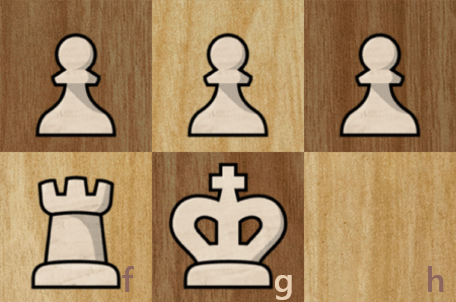
\includegraphics[height=5cm]{images/Chunk.png}
    \caption{Beispiel eines Chunks}
    \label{fig:chunk}
\end{figure}

Beim deklarativen Wissen im Schachkontext wird angenommen, dass Chunks eine zentrale Rolle spielen. Dabei handelt es sich um kleine Muster bzw. Anordnungen von einigen Spielfiguren, die öfter bei einem Schachspiel vorkommen. Ein Beispiel dafür könnte die Aufstellung in \autoref{fig:chunk} sein. Dort ist eine Position zu sehen, die häufig nach einer Rochade entsteht. Ein geübter Spieler erkennt dieses Muster sofort und weiß, dass der König relativ sicher ist. Es wird geschätzt, dass das Kurzzeitgedächtnis Platz für ungefähr sieben Chunks hat. Ein großer Unterschied zwischen geübten und weniger geübten Schachspielern ist, wie viele sie in ihrem Langzeitgedächtnis haben. Je besser ein Schachspieler ist, desto mehr und desto größere befinden sich in seinem Langzeitgedächtnis. Es wird vermutet, dass ein geübter Spieler ungefähr 50.000 Chunks in seinem Langzeitgedächtnis hat. Wenn ein Muster erkannt wird, muss im Kurzzeitgedächtnis nur ein Zeiger auf den Chunk im Langzeitgedächtnis behalten werden. Auf diese Weise können sich geübte Schachspieler sehr effizient Schachpositionen merken. Das erklärt auch, warum sich diese Fähigkeit nicht auf Bereiche außerhalb des Schachs auswirkt. Selbst zufällig angeordnete Positionen, die in regulären Spielen selten vorkommen, können sich gute Spieler schlecht merken. Erweitert wird diese Theorie durch Templates, also Vorlagen. Templates sind spezielle Chunks, welche Platzhalter für bestimmte Figuren beinhalten. Eine Template kann also auch angewendet werden, wenn sich vereinzelte Figuren an einer anderen Position befinden. So können durch Templates noch mehr Positionen abgedeckt werden, als es durch einfache Chunks möglich ist. Viele Chunks und Templates reduzieren die Notwendigkeit voraus zu schauen. Wenn bekannten Chunks begegnet wird, ist auch klar, wie gut diese Position zu bewerten ist und welche Züge in Frage kommen.
\cite{gobet_templates_1996}

Dieses Wissen, was als nächstes getan werden kann, wird von Gobet und Jansen unter dem prozedurales Wissen eingeordnet. Es wird durch sogenannte Produktionen abgespeichert. Produktionen sind Wissenseinheiten, welche aus Bedingung und Aktion bestehen. Ein Beispiel wäre, \enquote{Wenn es eine Linie ohne Figuren gibt und du einen Turm besitzt, dann platziere den Turm auf dieser Reihe.} Durch diese Produktionen können Spieler schnell Entscheidungen treffen. Dieser Mechanismus kann bewusst oder unbewusst stattfinden und wird oft als Intuition verstanden.
\cite{gobet_training_2006}

\subsection{Erlernen von Eröffnungen}
Das Lernen von Eröffnungen ist sehr zeitaufwendig. Es wird vermutet, dass sieben bis 10 Sekunden benötigt werden um einen Chunk im Langzeitgedächtnis zu lernen. Zudem ist es unvermeidlich, dass bestimmte Inhalte wieder vergessen werden. Deshalb wird empfohlen, sich auf wenige Eröffnungen zu konzentrieren. Für diese Eröffnungen können anschließend die häufigsten Variationen und Positionen erlernt werden.
Die Anzahl der Variationen solte so gewählt werden, dass auf typische Züge des Gegners reagiert werden kann.
Durch die begrenzte Anzahl der Eröffnungen, erhöht man die Wahrscheinlichkeit, dass gelernte Chunks und Templates in einem richtigen Spiel wiedererkannt werden. Beim Erlernen von Eröffnungen ist es außerdem wichtig eine Balance zwischen Auswendiglernen und Verständnis zu finden. Um sich die Abfolge der Züge zu merken muss man selbstverständlich viel Auswendiglernen, allerdings ist das Verständnis der Hauptideen nützlich um auch in unbekannten Situationen sinnvolle Züge zu finden. Dazu kommt, dass das Herausfiltern von Hauptideen, wie in \autoref{gedächtnis} beschrieben auch eine Lerntechnik ist, die beim Übertragen von Inhalten in das Langzeitgedächtnis helfen kann. Man sollte die Eröffnungen auch aus unterschiedlichen Perspektiven betrachten und Verknüpfungen zu Mittelspielen und Endspielen herstellen. Das soll die Erstellung von Templates beschleunigen. Ein zentraler Ort um die Eröffnungen nachzuschauen ist auch sinnvoll. Damit kann wird das Wissen einfach erneuert und es wird verhindert, dass die Erinnerungen verblassen oder sich verfälschen, wie in \autoref{gedächtnis} beschrieben.
\cite{gobet_training_2006}

Für eine Schachanwendung bedeutet das, dass Spieler ermutigt werden sollten eine Eröffnung und ihre Variationen im Detail zu erlernen. Außerdem sollten sie die Eröffnungen oft betrachten.
Hier kann die Schachanwendung selbst der zentrale Ort werden um Eröffnungen nachzuschauen und seine Erinnerung aufzufrischen. Um die Verknüpfungen zwischen Eröffnungen und Mittelspielen herzustellen kann dem Spieler die Möglichkeit gegeben werden, von einer bestimmten Eröffnung als Startpunkt gegen einen Computergegner zu spielen. Für die Verknüpfung von Eröffnungen und Endspielen kann die von Gobet und Jansen \cite{gobet_training_2006} vorgeschlagene Dekompositionsmethode verwendet werden. Hierbei werden nach der Eröffnung fast alle Figuren außer den Bauern und Königen vom Spielfeld entfernt. Dadurch bekommt man ein besseres Gefühlt dafür, welche Seite eine bessere Position hat. Man kann nach der Dekomposition den Spieler auch von dieser Position aus gegen einen Computer spielen lassen. Das Verstehen der Hauptideen von Eröffnungen kann durch beschreibende Infotexte erreicht werden. Auf diese Weise werden alle zuvor beschriebenen Bereiche abgedeckt. 

\subsection{Lernunterstützende Medien}
Es gibt viele Möglichkeiten das Lernen von Schacheröffnungen unterstützen. Heutzutage hat man viele Medien zur Auswahl, wie Bücher, Online Kurse, Videos oder Computerprogramme. Gobet und Jansen schreiben, dass die Reihenfolge und Art, wie Lernmaterial aufgeteilt wird essentiell für effektives Training ist. Sie empfehlen, dass eine lernende Person das nicht selbst auswählen sollte. Es sei wichtig, einen guten Trainer, gute Computerprogramme oder ein gutes Buch zu haben \cite{gobet_training_2006}.

Bücher waren lange Zeit das einzige und damit das Hauptmedium, über das Schachwissen übertragen wurde. Gobet und Jansen kritisieren, dass viele Bücher keinen psychologischen und pädagogischen Prinzipien folgen. Die meisten Bücher würden Schema nur anhand einer kleinen Anzahl an Positionen präsentieren. Außerdem seien Diagramme zu selten vorhanden \cite{gobet_training_2006}. Für Anfänger kann es schwierig sein anhand der textuellen Notation der Züge dem Text zu folgen. Ein Vorteil von Büchern ist, dass sie viel Hintergrundinformationen geben können. Sie können die langfristigen Ziele gut beschreiben und Kernideen erklären.

Ein Trainer kann einen genauen Trainingsplan für Lernende vorbereiten.
Seine Erfahrung hilft ihm dabei, das richtige Material auszuwählen und zu wissen welche Methoden effektiv sind.
Er kann die Schwächen eines Spielers erkennen und zielgerichtet Übungen vorbereiten um diese auszubessern. Auch das persönliches Feedback und Ratschläge können sehr hilfreich sein. Die Notwendigkeit eines Trainers ist umstritten, doch wenn man die Möglichkeit hat mit einem Trainer zu lernen, ist es wahrscheinlich die beste Option.
\cite{gobet_training_2006}

Es existiert bereits eine beachtliche Anzahl an Computerprogrammen, die einem Schachspieler eine umfangreiche Lernerfahrung bieten, oder ihn beim Lernen unterstützen können. Es gibt Plattformen mit Erklärvideos, interaktiven Lektionen und anschließenden Übungsaufgaben. Viele Webseiten bieten Puzzles und andere Taktikaufgaben an um sein Können zu trainieren. Auf Online Plattformen kann man auch über das Internet gegen andere Spieler spielen, die ein ähnliches Können haben. Computergegner bieten eine gute Möglichkeit neue Ideen auszuprobieren und seine Taktik zu verbessern. Mithilfe von Computeranalysen können Schwächen im eigenen Spiel ausgemacht werden und mithilfe von Spieldatenbanken können häufig gespielte Variationen genauer analysiert werden.

Auch Gobet und Jansen sehen das Potential für computergestütztes Lernen. Sie erwähnen die Nützlichkeit von Spieldatenbanken, Computergegnern und Analysen. Sie beschreiben auch, dass zukünftige Computerprogramme noch weitergehen können, indem sie wie ein Trainer personalisiert Übungsmaterial basierend auf den Stärken und Schwächen des Spielers heraussuchen.
\cite{gobet_training_2006} 

Gusev verwendet auch Computer, um auf Schacheröffnungen vorzubereiten. In \cite{gusev_using_2021} zählt er verschiedene Softwareprodukte auf, die beim Erlernen von Schacheröffnungen helfen können. Darunter sind Schachengines, Spieldatenbanken, Cloud Services und Puzzles. Er präsentiert eine computerbasierte Herangehensweise um Eröffnungen zu trainieren. Dafür identifiezierte und sortierte er mithilfe von Schachengines, Spieldatenbanken und einem Cloud Service beliebte Eröffnungsvarianten. Mögliche Fortführungen wurden durch eine Schachengine mit Eröffnungsbuch herausgefunden. Das Resultat war ein nützliches Werkzeug, um Lerndenden Eröffnungen zu zeigen.

\section{Funktionsweise von Schachengines}
Seit langer Zeit wird die Fähigkeit Schach zu spielen mit Intelligenz verbunden.
Daher gab es auch großes Interesse daran Computern das Spielen von Schach beizubringen.
Es wurden Preise ausgeschrieben für die Programme, die als erstes eine bestimmte Wertung erreichen oder den Weltmeister besiegen. Das erste Mal, dass ein Computer einen Weltmeister besiegte war im Jahr 1997. Das von IBM entwickelte Programm namens \enquote{Deep Blue} besiegte den aktuellen Weltmeister Garry Kasparov. Seitdem ist die Lücke zwischen Menschen und Computern immer größer geworden und heutzutage kann kein Mensch mehr gegen die besten Schachcomputer gewinnen.
\cite{vjekoslav_nemec_history_2019}

Computerprogramme, die Schach spielen werden typischerweise Schachengines genannt. Es gibt unterschiedliche Formen von Schachengines. Die einen nutzen den Minimax"=Algorithmus in Verbindung mit Alpha-Beta-Pruning. Das ist auch die Art von Schachengines, die zuerst entwickelt wurden. Eine weitere Form wurde in den letzten Jahren entwickelt. Diese arbeiten mit reinem Reinforcement Learning und erlernen das Spiel, indem sie zahlreiche Spiele gegen sich selbst spielen. In den Folgenden zwei Kapiteln werden beide Herangehensweisen näher erläutert.

\subsection{Alpha-Beta-Pruning}
Der Alpha-Beta-Pruning Algorithmus kann genutzt werden um ein Spiel mit zwei Spielern, die gegensätzliche Ziele verfolgen, zu spielen. Der Algorithmus baut auf dem Minimax Algorithmus auf und optimiert diesen durch Kürzen (Pruning) des Suchbaums.

Für den Minimax Algorithmus wird ein Spiel anhand von Positionen $p$ und von Regeln, wie von einer Position in eine andere übergegangen werden kann definiert. Wenn es keine weiteren legalen Züge gibt, ist eine Terminalposition erreicht. Diese Struktur kann als sogenannter Spielbaum dargestellt werden. Die Positionen bilden die Knoten und wenn ein Übergang von einer Position in eine andere existiert, wird eine Kante eingezeichnet. Falls eine Position schon einmal erreicht wurde darf allerdings keine Kante hinzugefügt werden um Zyklen zu verhindern. Bei diesem Baum ist $h$ die Tiefe des Baumes und $d$ ist die Anzahl an Verzweigungen an einem Knoten. Die Terminalpositionen bilden die Blattknoten.
\cite{knuth_analysis_1975}

Jeder Terminalposition wird ein Wert zugewiesen durch die Evaluationsfunktion $f(p)$. Für einen Spieler ist der Wert des Spiels $f(p)$ und für den anderen der Wert $-f(p)$. Beide Spieler möchten jeweils ihren Wert maximieren. Alternativ kann man auch formulieren, dass ein Spieler den Wert von $f(p)$ maximieren will und der Gegner will ihn minimieren.
Beide Herangehensweisen sind äquivalent. Wenn $p$ eine Position ist, bei der es es $d$ legale Züge $p_1,\ldots,p_d$ mit $d > 1$ gibt, dann ist es die Aufgabe des Algorithmus, den besten Zug auszuwählen. Der beste Zug ist der Zug, bei dem der beste Wert für den Spieler am Zug erreicht wird. Es wird davon ausgegangen, dass der Gegner auch jeweils die Züge auswählt, die für ihn zu dem besten Wert führen. Es sei $F(p)$ der größtmögliche Wert, der von Position $p$ aus erreichbar ist gegen einen optimal spielenden Gegner. Die Funktion $F(p)$ wird definiert durch:
\begin{equation*}
    F(p) = 
    \begin{cases}
        f(p) & \text{für } d = 0 \\
        max(-F(p_1),\ldots,-F(p_d)) & \text{für } d > 0
    \end{cases}
\end{equation*}

Mit Pseudocode kann diese Funktion folgendermaßen abgebildet werden:
\begin{lstlisting}[caption=Minimax-Algorithmus,label=lst:minmax]
function F(p: Position): Int {
    ps = findSuccessors(p)
    d = ps.length
    if (d == 0) {
        return f(p)
    }
    m = -infinity
    for (pi in ps) {
        t = -F(pi)
        m = max(t, m)
    }
    return m
}
\end{lstlisting}

Dieser Algorithmus durchsucht alle Möglichen Fortsetzungen von $p$ und findet den Zug mit dem besten Wert. 
\cite{knuth_analysis_1975}

Es ist allerdings nicht immer notwendig alle Fortsetzungen zu zu überprüfen. Oft kann erkannt werden, dass eine bestimmte Zugfolge keinen besseren Wert mehr erreichen kann und daher ignoriert werden kann.
Wenn man zum Beispiel eine Zugfolge herausgefunden hat, die mit dem Wert 3 bewertet wird und man über eine andere Zugfolge sagen kann, dass diese nicht besser als 3 wird, muss man diese nicht weiter nachverfolgen. Wenn also $-F(p_1) = 3$ ist, dann ist $F(p) \geq 3$ und jeder Pfad für den $-F(p_i) \leq 3$ gilt, kann ignoriert werden.
Der Gegner kann in diesem Fall den Zug so wählen, dass entweder derselbe Wert oder ein für uns kleinerer Wert erzielt wird. Indem man den aktuell höchsten Wert zwischenspeichert, ist es möglich bestimmte Suchzweige auszulassen.
\cite{knuth_analysis_1975}

Dieses Vorgehen kann weiter verbessert werden indem man den höchsten und den kleinsten Wert zwischenspeichert. Das wird Alpha-Beta-Pruning genannt. Knuth und Moore definieren die Funktion $F2$ folgendermaßen:

\begin{equation*}
    \begin{array}{ll}
        F2(p, \alpha, \beta) \leq \alpha & \text{für }F(p) \leq \alpha \\
        F2(p, \alpha, \beta) = F(p) & \text{für }\alpha < F(p) < \beta \\
        F2(p, \alpha, \beta) \geq \beta & \text{für }F(p) \geq \beta
    \end{array}
\end{equation*}

In Pseudocode kann der Algorithmus folgendermaßen umgesetzt werden:
\begin{lstlisting}[caption=Alpha-Beta-Pruning,label=alphabeta]
function F2(p: Position, alpha: Int, beta: Int): Int {
    ps = findSuccessors(p)
    d = ps.length
    if (d == 0) {
        return f(p)
    }
    m = alpha
    for (pi in ps) {
        t = -F2(pi, -beta, -m)
        m = max(t, m)
        if (m >= beta) break
    }
    return m
}
\end{lstlisting}

Für diesen Algorithmus können weitere Verbesserungen vorgenommen werden. Einen großen Faktor spielt die Reihenfolge, in der die Züge untersucht werden. Bei einer optimalen Reihenfolge muss der Alpha-Beta-Algorithmus $d^{\lceil h/2 \rceil} + d^{\lfloor h/2 \rfloor} - 1$ Terminalpositionen bewerten \cite{knuth_analysis_1975}. Das ist dann der Fall, wenn beim Durchsuchen des Baumes immer der richtige Zug ausgewählt wird, sodass er maximal gekürzt werden kann. Der Algorithmus kann dahingehend verbessert werden, dass Züge, die mit hoher Wahrscheinlichkeit einen Vorteil bringen zuerst betrachtet werden. Im Schach können zum Beispiel Züge in welchen eine Figur geschlagen wird zuerst betrachtet werden, da diese oft einen Vorteil bringen. Andere Züge, wie zum Beispiel Damenopfer können später betrachtet werden.
Um die Reihenfolge der Züge für eine tiefere Suche zu verbessern, wird häufig zunächst eine flachere Suche durchgeführt. Dieses Verfahren wird als iterative Vertiefung (iterative deepening) bezeichnet. 
Eine optimale Reihenfolge kann man dadurch jedoch nicht garantieren. Wie in der Gleichung zu sehen ist steigt die Anzahl der zu besuchenden Knoten selbst im Optimalfall exponentiell. Es kann also nur eine bestimmte Anzahl an Zügen in die Zukunft geschaut werden. Für viele Spiele, einschließlich Schach, ist die Gesamtzahl der möglichen Züge in einem Spiel jedoch so hoch, dass es mit heutigen Mitteln nicht möglich ist, alle Szenarien vollständig zu analysieren. Aus diesem Grund wird eine bestimmte Suchtiefe festgelegt, ab der die Positionen wie Terminalpositionen behandelt werden \cite{knuth_analysis_1975}. Es muss also für diese Position auch eine Evaluationsfunktion $f$ existieren. In der naivsten Form kann dafür die Anzahl der Figuren der Spieler genommen werden. In komplexeren Schachengines werden Neurale Netze verwendet um Positionen zu bewerten. Eine Tabelle mit bereits berechneten Positionen kann Berechnungen auch beschleunigen. Für Eröffnungen und Endspiele können Eröffnungsbücher und vorgerechnete Endspiel Tabellen verwendet werden \cite{silver_mastering_2017}.

\subsection{Reinforcement Learning}\label{cp:alphazero}
Der klassische Alpha-Beta-Pruning Algorithmus kann nur durch viel spielbezogenes Wissen verbessert werden. Im Gegensatz dazu kann im Reinforcement Learning ein Computer ein Spiel ohne Vorwissen erlernen, indem er wiederholt Spiele gegen sich selbst simuliert. Das bekannteste Beispiel dafür ist AlphaZero, ein Algorithmus, der nach wenigen Stunden Training die besten Programme für Schach, Shogi und Go schlagen konnte. \cite{silver_mastering_2017} In diesem Kapitel wird die Funktionsweise von AlphaZero näher erklärt.

AlphaZero basiert auf dem Algorithmus AlphaZero Go, welcher der erste ist, der Go auf einem \enquote{superhuman level}\cite{silver_mastering_2017-1} spielen kann. Einige Verbesserungen, die speziell für Go waren, wurden dafür weggelassen.\cite{silver_mastering_2017} Beide Algorithmen verwenden ein Deep Neural Network im Zusammenhang mit der \ac{MCTS}.

Bei \ac{MCTS} wird ein Suchbaum inkrementell aufgebaut bis ein Rechenlimit erreicht wird. Dieses Rechenlimit wird meistens durch eine Zeitbegrenzung realisiert. Es wird also für eine bestimmte Zeit ein Suchbaum aufgebaut, dann abgebrochen und der bis dahin beste gefundene Wert ausgegeben. Dieses Verfahren ist sehr effizient für Bäume mit hoher Verzweigung. In diesem Verfahren werden bereits bekannte Knoten durch eine Baumstrategie (Tree Policy) ausgewählt und sobald ein Knoten mit unbekannten Kindesknoten erreicht wird, wird die Standardstrategie (Default Policy) angewendet. Bereits besuchte Knoten besitzen eine Bewertung und die Anzahl, wie oft sie besucht wurden. Eine Tree Policy muss die Knoten so auswählen, dass vielversprechende Knoten besucht werden und auch neue Pfade erkundet werden. Es gilt also eine Balance zu finden zwischen gut bewerteten Knoten und selten besuchten Knoten. Der Erfolgt von \ac{MCTS} hängt zu großen Teilen von dieser Tree Policy ab. Ein Verfahren, was sich als erfolgreich herausgestellt hat ist der \enquote{upper confidence bound for trees (UCT)} Algorithmus, welcher hier nicht näher erläutert wird \cite{browne_survey_2012}. Bei einem Knoten mit unbekannten Kindesknoten wird ein Spiel mithilfe der Default Policy simuliert, bis ein Terminalknoten erreicht wird. Der Terminalknoten kann mit einem Belohnungswert bewertet werden. Dieser Belohnungswert wird zurückpropagiert und die Bewertungen der vorhergegangen Knoten werden angepasst. Im einfachsten Fall kann die Default Policy eine gleichmäßige Zufallsverteilung sein. Die Züge werden also zufällig ausgewählt.
\cite{browne_survey_2012}

Bei AlphaZero wird \ac{MCTS} mit einem tiefen Neuralen Netz $f_\theta$ mit den Paramtern $\theta$ verwendet. Dieses Netz bekommt die aktuelle Position $s$ als Eingabe und gibt einen Vektor $p$ und einen Skalar $v$ aus $(p, v) = f_\theta(s)$. Der Vektor $p$ gibt die Wahrscheinlichkeit an, dass ein bestimmter Zug ausgewählt wird. Der Skalar $v$ schätzt die Wahrscheinlichkeit, dass der Spieler am Zug mit der aktuellen Position gewinnen wird. AlphaZero wird durch Reinforcement Learning trainiert indem es wiederholt gegen sich selbst spielt. Für jede Position $s$ wird eine \ac{MCTS} Suche durchgeführt, welche durch das Neurale Netz $f_\theta$ geführt wird. Die Ausgabe dieser Suche sind die Zugwahrscheinlichkeiten $\pi$ und der Gewinner $z$. Diese Wahrscheinlichkeiten sind deutlich besser, als die Ausgaben des Neuralen Netzes. Die Parameter des neuralen Netzes werden angepasst, sodass der Unterschied zwischen $(p, v) = f_\theta(s)$ und $(\pi, z)$ möglichst gering wird. Konkret werden die Parameter $\theta$ durch den Gradientenabstieg auf einer typischen Verlustfunktion angepasst.
\cite{silver_mastering_2017-1,silver_mastering_2017}

Der beschriebene Algorithmus wurde jeweils für Schach, Shogi und Go trainiert. In Schach und Shogi spielte AlphaZero nach weniger als einem Tag Training besser als die bis dahin führenden Programme. Im Vergleich zu Alpha-Beta-Pruning Algorithmen, wie zum Beispiel Stockfish durchsucht AlphaZero deutlich weniger Pfade pro Sekunde. Das ganze wird dadurch kompensiert, dass AlphaZero bei der Auswahl der zu untersuchenden Pfade selektiver vorgeht. Es wurde auch gezeigt, dass AlphaZero mit mehr Bedenkzeit effizienter skaliert. Des weiteren werden Fehler in der Schätzung von Positionen durch \ac{MCTS} geschwächt, während sie bei Alpha-Beta-Pruning Algorithmen bis zur Wurzel wandern.
\cite{silver_mastering_2017}

\section{Schnittstellen}
Damit Schachengines in andere Programme eingebunden werden können sind Schnittstellen notwendig.
Das zu entwickelnde Programm soll ein Backend für eine Schachlernanwendung im Web bilden. Dafür muss es zum einen eine Schachengine einbinden und ihre Schnittstelle ansteuern und zum anderen Schnittstellen, für eine Weboberfläche zur Verfügung stellen.
%Das zu entwickelnde Programm muss also eine Schnittstelle ansteuern können, die die Schachengine unterstützt. Zusätzlich wird eine Schnittstelle benötigt um mit einer Weboberfläche zu kommunizieren un dem Nutzer eine Benutzeroberfläche bereitzustellen. 
Schnittstellen zwischen Programmen werden \ac{API} genannt. Sie erlauben es unterschiedlichen Programmen miteinander zu kommunizieren und interagieren. Die Programme können dabei mit unterschiedlichen Technologien erstellt word sein und auch auf verschiedenen Rechnern ausgeführt werden, solange sie sich durch eine gemeinsame \ac{API} verständigen können.
In den folgenden Kapiteln wird beschrieben, wie die Schnittstelle zu einer Schachengine meistens gestaltet wird und wie Schnittstellen zwischen einer Weboberfläche und dem Backend gebildet werden können.

\subsection{Schachengine Schnittstellen}
Heutzutage unterstützen die meisten Schachprogramme das \ac{UCI}. Es hat fast vollständig das ältere Protokoll XBoard ersetzt. Der primäre Zweck des Protokolls ist es eine Engine mit einer GUI zu verbinden. Die Aufgabe der GUI ist es dabei nicht nur eine Benutzeroberfläche dazustellen, sondern auch den Zustand zu speichern. Das ermöglicht es, dass die Engine zustandslos ist und reduziert somit ihre Komplexität. Die GUI kann auch Züge von einem Eröffnungsbuch oder einer Endspieltabelle auswählen. Ein Format für die Eröffnungsbücher wird nicht vorgeschrieben. Sie können je nach GUI Programm variieren. Diese Aufgabe muss nicht in der Engine erledigt werden.
\cite{wikipedia_foundation_inc_universal_2024}

Die Kommunikation findet bei diesem Protokoll über die Standardeingabe und Standardausgabe der Konsole statt. In dem Protokoll sind einige Kommandos definiert, über die eine GUI Daten abfragen und setzen kann und Aktionen starten. Ein typischer Ablauf kann folgendermaßen aussehen:
\begin{enumerate}
    \item Die GUI schickt zur Initialisierung das Kommando \lstinline{uci}.
    \item Die Engine antwortet mit ihrem Namen, Autor und den Optionen, die eingestellt werden können.
    \item Wenn alle Informationen gesendet wurden schickt sie \lstinline{uciok}
    \item Jetzt kann die GUI mit dem Kommando \lstinline{setoption} Optionen setzen.
    \item Mit dem Kommando \lstinline{isready} kann überprüft werden, ob die Engine bereit ist für den nächsten Schritt.
    \item \lstinline{ucinewgame} startet ein neues Spiel.
    \item Die Position wird mit dem Kommando Position gesetzt, z. B. \lstinline{position startpos moves e2e4 e7e5}. Statt \lstinline{startpos} kann auch ein FEN-String übergeben werden. Das ist eine String Darstellung der aktuellen Position. Nach \lstinline{moves} können die gespielten Züge in algebraischer Notation dargestellt werden. Dabei beschreiben die ersten zwei Zeichen die ursprüngliche Position der Figur und letzten zwei den Zielort. e2e4 bewegt also eine Figur von der Position e2 zur Position e4. Da die Position davor die Startposition war, muss es ein Bauer gewesen sein.
    \item Mit dem Kommando \lstinline{go} startet die Engine die Berechnung. Diesem Kommando können auch Begrenzungen mitgegeben werden, wie zum Beispiel die maximale Tiefe oder maximale Anzahl an Knoten, die untersucht werden sollen.
    \item Während der Berechnung gibt die Engine kontinuierlich Zwischeninformationen über die aktuelle Tiefe untersuchten Züge und weitere Parameter.
    \item Die GUI kann die Berechnung jederzeit beenden mit dem Kommando \lstinline{stop}.
    \item Wenn die Berechnung beendet ist oder durch \lstinline{stop} abgebrochen wurde, sendet die Engine den besten herausgefundenen Zug mit dem Kommando \lstinline{bestmove}.
\end{enumerate}
\cite{stefan_meyer-kahlen_universal_2025}

\subsection{Web-Schnittstellen}
Die Benutzerschnittstelle für dieses Projekt soll als Weboberfläche realisiert werden. Dafür wird es in zwei Bestandteile aufgeteilt, das Backend und das Frontend. Damit diese Bestandteile miteinander kommunizieren können, ist es notwendig eine \ac{API} zur Kommunikation zu entwickeln.

Für diesen Anwendungsfall werden häufig \ac{REST}ful APIs erstellt. \ac{REST} ist eine Architektur, die HTTP verwendet, um zwei Systeme miteinader kommunizieren zu lassen. Damit eine API als \ac{REST}ful bezeichnet werden kann, müssen einige Prinzipien oder auch Einschränkungen eingehalten werden.

\subsubsection{REST-Prinzipien}

REST-APIs sind Client-Server-Architekturen. Dahinter steckt das Prinzip der Separierung von Anliegen (separation of concerns). Das hat den Vorteil, dass der Client und Server gegenseitig nichts über ihre Technologien und Implementierungen wissen müssen und separat entwickelt werden können. Auch bei diesem Projekt werden Client und Server separat entwickelt.

Ein Kernaspekt von REST-APIs ist, dass sie zustandslos sind. Der Server muss sich den Zustand des Clients nicht merken. Stattdessen liegt es in der Verantwortung des Clients, bei jeder Anfrage den aktuellen Kontext mitzusenden. Das ist auch der Fall bei mehrteiligen Anfragen. Die Zuverlässigkeit wird dadurch verbessert, da es einfacher ist, Fehlerzustände zu beheben. Die Skalierbarkeit ist auch verbessert, da die Aufgaben des Servers vereinfacht sind und Load Balancer einfacher zu implementieren sind.

Ein weiteres Rest-Prinzip ist das Caching. Daten einer Antwort werden implizit oder explizit als chachebar oder nicht cachebar markiert. Ein Client kann dann cachebare Antworten wiederverwenden für spätere äquivalente Anfragen. Das ermöglicht schnellere Antwortzeiten und kürzere Latenzen. Es kann allerdings die Zuverlässigkeit beeinträchtigen.

REST-APIs sind in hierarchischen Schichten organisiert. Eine einzelne Schichten sind voneinander gekapselt. Das reduziert die Komplexität des Systems, da verschiedene Bestandteile separat betrachtet werden können. Die Schichten können auch auf verschiedene Prozesse oder Systeme verteilt sein. An den Schichtgrenzen können gemeinsame Caches genutzt werden und es können Sicherheitsregeln zwischen den Schichten definiert werden. Das kann die Sicherheit des Systems erhöhen. Ein Nachteil ist, dass die Schichtenarchitektur Overhead hinzufügt und die Latenz erhöhen kann. Dass kann allerdings durch die Verwendung von Chaches ausgeglichen werden.

Eine REST-API hat eine einheitliche Schnittstelle. Das hilft dabei die Kommunikation zwischen den Komponenten zu definieren. Es entkoppelt die Kommunikation von der Architektur. Jede Ressource hat eine eindeutige URI über die man auf sie zugreifen kann. Das Frontend muss nicht wissen, wie die Daten abgespeichert sind. Sie werden mit einem portablen Format, wie XML oder JSON verschickt.

Eine optionale Anforderung an REST-APIs ist code-on-demand. Das beschreibt die Möglichkeit den Client durch das Herunterladen von Applets oder Skripten zu erweitern.
\cite{fielding_architectural_2000,de_api_2017}

\subsubsection{URI Design}
In REST-APIs werden Ressourcen über \ac{URI}s identifiziert. Sie bestehen aus dem Protokoll, der Webadresse und darauffolgend einem Pfad, z. B. \lstinline[language={}]{https://api.example.com/path}. Für REST-APIs gibt es einige Regeln und Best-Practices, wie der Pfad von \ac{URI}s gestaltet wird.

Die erste Regel ist, dass der Schrägstrich dazu genutzt werden soll, eine hierarchische Struktur darzustellen. Zum Beispiel könnten Eröffnungen folgendermaßen angordnet sein: \lstinline{/openings/queens-gambit}. Das Queen's Gambit ist eine Eröffnung, deshalb ist sie unter der Ressource \lstinline{openings} platziert.

In dem vorherigen Beispiel sind auch weitere Regeln zu sehen. Um die Lesbarkeit zu erhöhen, werden Bindestriche verwendet. Unterstriche werden vermieden, da sie in Links oft schlecht oder gar nicht sichtbar sind. Außerdem sollen Pfade ausschließlich Kleinbuchstaben enthalten, um Verwirrung zu vermeiden.

In REST-APIs gibt es vier verschiedene Arten von Daten, die ihre eigenen Namenskonventionen besitzen.

Dokumente (documents) sind einzelne Ressourcen, wie zum Beispiel eine einzelne Objektinstanz oder ein Datenbankeintrag. Diese werden mit einem Substantiv oder einer Nominalphrase benannt. Auch das ist in dem Queen's Gambit Beispiel zu sehen. \lstinline{queens-gambit} ist hier das Substantiv.

Sammlungen (collections) sind Verzeichnisse von Ressourcen, die durch den Server verwaltet werden. Clients können neue Elemente für diese Verzeichnisse vorschlagen, der Server entscheidet, ob das Element hinzugefügt wird. Eine Sammlung wird mit einem Substantiv im Plural oder einer Nominalphrase benannt. Ein Beispiel ist der Pfad \lstinline{/openings}, welcher eine Sammlung von Eröffnungen enthält.

Ein Speicher (store) ist ein Speicherort, der vom Client verwaltet wird. Ein Anwendungsfall kann ein Client sein, der die Dokumentenressource \lstinline{queens-gambit} in seinen Speicher \lstinline{favorites} speichert. \lstinline{PUT /users/1234/favorites/queens-gambit}

Controller stellen ausführbare Funktionen mit Parametern und Rückgabewerten dar.
Darunter fallen Aktionen, die sich nicht eindeutig den klassischen CRUD-Operationen – also Erstellen (Create), Lesen (Read), Aktualisieren (Update) oder Löschen (Delete) – zuordnen lassen.
Cotroller sind meistens das letzte Element in der Hierarchie und besitzen keine Kindelemente. Benannt werden sie mit einem Verb oder einer Verbalphrase. Ein Beispiel wäre eine Controllerressource, die es einem Client erlaubt eine Meldung erneut zu senden: \lstinline{/alerts/2345/resend}.

\ac{URI}s sollten keine CRUD-Funktionen in ihren Namen verwenden. Stattdessen sollten HTTP Methoden zeigen, welche CRUD-Operation ausgeführt wird. Die CRUD-Funktionen einer Userressource können folgendermaßen aussehen:

\begin{itemize}
  \item Create user $\rightarrow$ \lstinline{POST oder PUT /users}
  \item Receive user $\rightarrow$ \lstinline{GET /users}
  \item Update user $\rightarrow$ \lstinline{PATCH /users/2345}
  \item Delete user $\rightarrow$ \lstinline{DELETE /users/3423}
\end{itemize}

In \ac{URI}s kann es Pfadsegmente geben die statisch oder dynamisch sind. Statische Pfadsegmente sind unveränderliche Namen, die durch einen Designer im Voraus festgelegt werden. Dynamische Pfadsegmente sind veränderlich und erfüllen meist den Zweck eines Identifikators, der aus einer Sammlung oder einem Speicher ein Element identifiziert. Im folgenden Beispiel ist das Pfadsegment \lstinline{openings} statisch und das Segment \lstinline|{id}| ist dynamisch und wird vor der Ausführung durch eine konkrete Eröffnungs-ID ersetzt: \lstinline|/openings/{id}|

Nach dem Pfad können noch weitere Query-Parameter definiert werden. Diese sind dazu da um Sammlungen oder Speicher zu filtern. Folgende Query könnte genutzt werden um alle Eröffnungen zu bekommen, die zur Familie Queen's Gambit gehören: \lstinline{GET /openings?family=queens-gambit}.
\cite{masse_rest_2012}

\subsubsection{Authentifizierung}
\label{cp:auth}
Authentifizierung ist der Prozess, bei dem die Identität eines Nutzers verifiziert wird.
Dieser Prozess ist in vielen APIs wichtig und muss sicher implementiert werden. Eine unsichere Authentifizierung ist eine große Sicherheitslücke, die es Dritten ermöglicht Zugriff zu Ressourcen zu erlangen, die ihnen nicht zustehen.
Es gibt viele Gründe, warum Authentifizierung benötigt wird. Einer davon ist, um nutzerbezogene Daten zu sammeln.
Auch in der Schachanwendung soll das geschehen, um eine personalisierte Erfahrung zu ermöglichen.
Einen Nutzer könnte zum Beispiel interessieren, welche Schacheröffnungen er bereits oft geübt hat. Außerdem ist es sinnvoll rechenintensive Operationen nur authentifizierten Nutzern zur Verfügung zu stellen. Das reduziert die Wahrscheinlichkeit eines \ac{DoS} Angriffs zu erliegen, bei der durch viele Anfragen der Server überlastet wird. Das Verwenden einer Schachengine ist zum Beispiel sehr rechenintensiv und sollte nur authentifizierten Nutzern erlaubt sein.

Authentifizierung lässt sich in drei Faktoren einteilen:
\begin{itemize}
    \item Wissensbasierte Authentifizierung erfolgt durch etwas, dass man weiß, wie zum Beispiel ein Passwort.
    \item Besitzbasierte Authentifizierung erfolgt durch etwas, dass man besitzt, wie zum Beispiel einen Schlüssel.
    \item Biometrische Authentifizierung erfolgt durch etwas, dass man ist, wie zum Beispiel wie der Fingerabdruck aussieht.
\end{itemize}

Auf Webseiten findet die erste Authentifizierung meistens wissensbasiert mithilfe eines Passworts statt. Bei der Erstellung des Accounts muss ein Nutzer ein Passwort angeben, das er bei erneutem Anmelden wieder angeben muss.
Um die Sicherheit dieses Verfahrens zu gewährleisten, darf die Übertragung des Passworts ausschließlich über eine verschlüsselte Verbindung (z.B. HTTPS) erfolgen. Außerdem dürfen Passwörter nicht in Klartext gespeichert werden, sondern müssen durch sichere Hashfunktionen umgewandelt werden. Diese Funktionen produzieren bei gleicher Eingabe die gleiche Ausgabe, es kann allerdings nicht durch die Ausgabe auf das Passwort zurückgeschlossen werden. Noch sicherer werden diese Funktionen, wenn vor der Anwendung ein Salt hinzugefügt wird, also eine zufällige Kombination von Zeichen.

Passwörter sollten nicht bei jeder Anfrage geschickt werden, da jede Anfrage, in der ein Passwort geschickt wird, auch ein gewisses Risiko birgt. Deshalb existiert die tokenbasierte Authentifizierung. Bei ihr wird am Anfang ein Login mit Passwort durchgeführt und der Client bekommt daraufhin ein Token. Dieses Token ist ein zufällig generierter String, den nur der Server und der Client kennt. Der Client kann sich damit also wissensbasiert authentifizieren. 

Für die genaue Verwendung von Tokens gibt es mehrere Möglichkeiten. Eine Möglichkeit ist das Token auf dem Server in einer Datenbank abzulegen, sodass dieser einen Client wiedererkennen kann. Um ein Token zu deaktivieren kann man es wieder aus der Datenbank entfernen. Auf dem Client kann man das Token in einem Cookie speichern und ihn auffordern das Token bei zukünftigen Anfragen zu verwenden. Die Technologie ist in den aktuellen Browsern gut unterstützt und daher auch leicht zu implementieren. Nachteilhaft bei diesem Vorgehen ist, dass der Server in diesem Fall Zustände speichern muss. Das wiederspricht dem Prinzip von REST-APIs, die per Definition zustandslos sein sollen. Die Überpüfung der Token mit einer Datenbank skaliert bei sehr vielen Nutzern auch nicht so gut und ist anfällig für Timing Attacken. Das bedeutet, dass ein Angreifer Token herausfinden kann anhand dessen, wie lange eine Anfrage benötigt.

Das Problem der Timing Attacken kann gelöst werden, indem die Nachrichten durch einen \ac{MAC} ergänzt werden. Das Token erhält also zusätzlich einen Code, der bestätigt, dass er von dem Server erstellt wurde. Dafür kann die \ac{HMAC}-Funktion genutzt werden. Diese Funktion erstellt unter Verwendung der Daten und eines geheimen Schlüssels den \ac{MAC}. Jede Veränderung der Daten führt zur Ungültigkeit des \ac{MAC}. Die Funktion kann nicht nur auf Tokens angewendet werden, sondern auf beliebige Daten. Im Endeffekt benötigt man auch keine Tokens mehr und die Informationen über die Berechtigungen können direkt an den Client übergeben werden, da sie vor Bearbeitung geschützt sind. Auf diese Weise funktionieren auch \ac{JWT}. Ein JSON-Objekt wird in Base64 umgewandelt und mithilfe einer \ac{HMAC}-Funktion signiert. Mit der selben Funktion kann bei späteren Anfragen getestet werden, ob die Daten unverändert sind. Wenn das der Fall ist muss der neu generierte \ac{MAC} mit dem vorhandenen übereinstimmen.
\cite{madden_api_2020,software_development_engineering_advisor_at_fiserv_usa_architecting_2023}

% Hier kann man noch mehr ins Detail gehen, wenn man will. Zum Biespiel Risiken und Nachteile mit JWTs.

